\Aufgabe{Karol mit Java und Struktogramme}

\doppelseite{0.55}{0.3}{t}{%
\begin{itemize}
    \item Bearbeite die Robot Karol (\url{karol.arrrg.de}) Level erneut. Schreibe den Programmcode dieses Mal direkt in Java!\\
    Zur Erinnerung: Deinen Code schreibst du an der gelb markierten Stelle in der main-Methode.
    \item Zeige nach den Schritten jeweils das Struktogramm an und notiere auf einem \emphColB{Schmierzettel}, wie du die letzte Spalte in Hefteintrag \ref{sec:befehlsarten} befüllen würdest.
    \item Was passiert, wenn du dein Programm aus eigenen Methoden aufbaust? Wieso ist das so?
\end{itemize}

}{%
 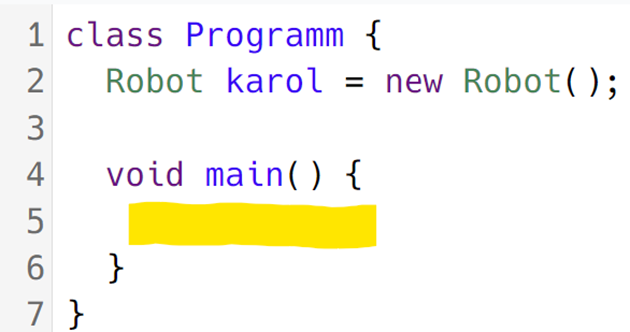
\includegraphics[width=\linewidth]{_Aufgaben/BlocklyJava_Skript/img/A04_karol_mainMarkiert.png}
 
 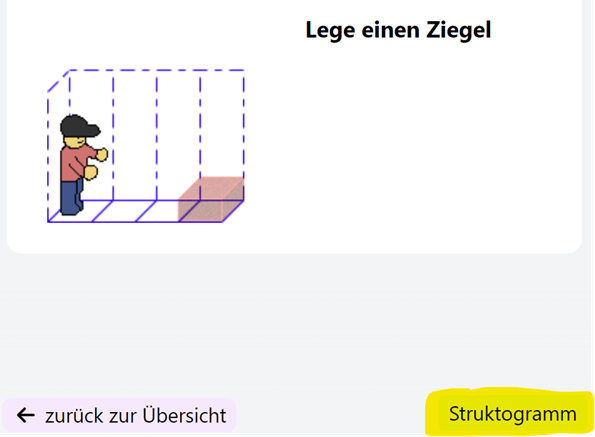
\includegraphics[width=\linewidth]{_Aufgaben/BlocklyJava_Skript/img/A04_karol_struktoMarkiert.png}
}

